%!TEX root = ../Thesis.tex

% To add:
% the one ephem data set can be used as all satellites send the same data for all otehr satellites


How to evaluate?:
- accuracy in relative space\\
- compare to just taking differences in absolute position \\
- between individual receivers and the total error in the whole system\\
- markov? error analysis -> cannot do precision without statistical analysis but isolate errors in x,y,z. how much worse is z than horizontal?\\
- computational time-> how does more receivers/satellites affect the comp time -> what time and space complexity?


\section{Evaluation}
Base Evaluation
In NED frame, have two receivers
- vary the distance by 0.1m, 1m, 10m ... 100km
- set it as x, y, z for each distance and satellite configuration
- Use 'fake' satellite positions?
Sat configs:
	- only sats in one orbit - 1D 
	- cluster directly above
	- cluster at the edges
	- sats in the same plane as the difference in receivers
	- 


- how close the 'approximate location' setting is to the alpha receiver

- what affect random errors have on the accuracy - use a time scale


- vary number of satellites in view\\
- vary GDOP (good GDOP and bad)\\
- when receivers don't see the exact same satellites \\
- vary number of receivers \\
- simulate a multipath error and how does it account for it or how much error does it introduce\\
\subsubsection{Fake Satellite Positions}
It is assumed that the orbits are circular, this is valid as the eccentricity (e) of the GPS satellites are all $e<10^{-3}$.  The eccentricity is a measure of how elliptical an orbit is; where e = 0 is a perfect circle and e = 1 is a parabola. It is also assumed that the Earth is circular and has a radius of 
$r_e = 6.378137\times10^6 m$.

\begin{eqnarray}
\sin\alpha = \frac{r_e\sin(\pi/2+\theta)}{a}\\
R = \frac{a\sin(\pi-(\pi/2+\theta)-\alpha)}{\sin\theta}\\
R = \frac{a\cos\left( \theta+\sin^{-1}\left( \frac{r_e\cos(\theta)}{a} \right) \right)}{\cos(\theta)}
\end{eqnarray}
\begin{figure}
\centering
\caption{text}
\label{fig:orbit_distance}
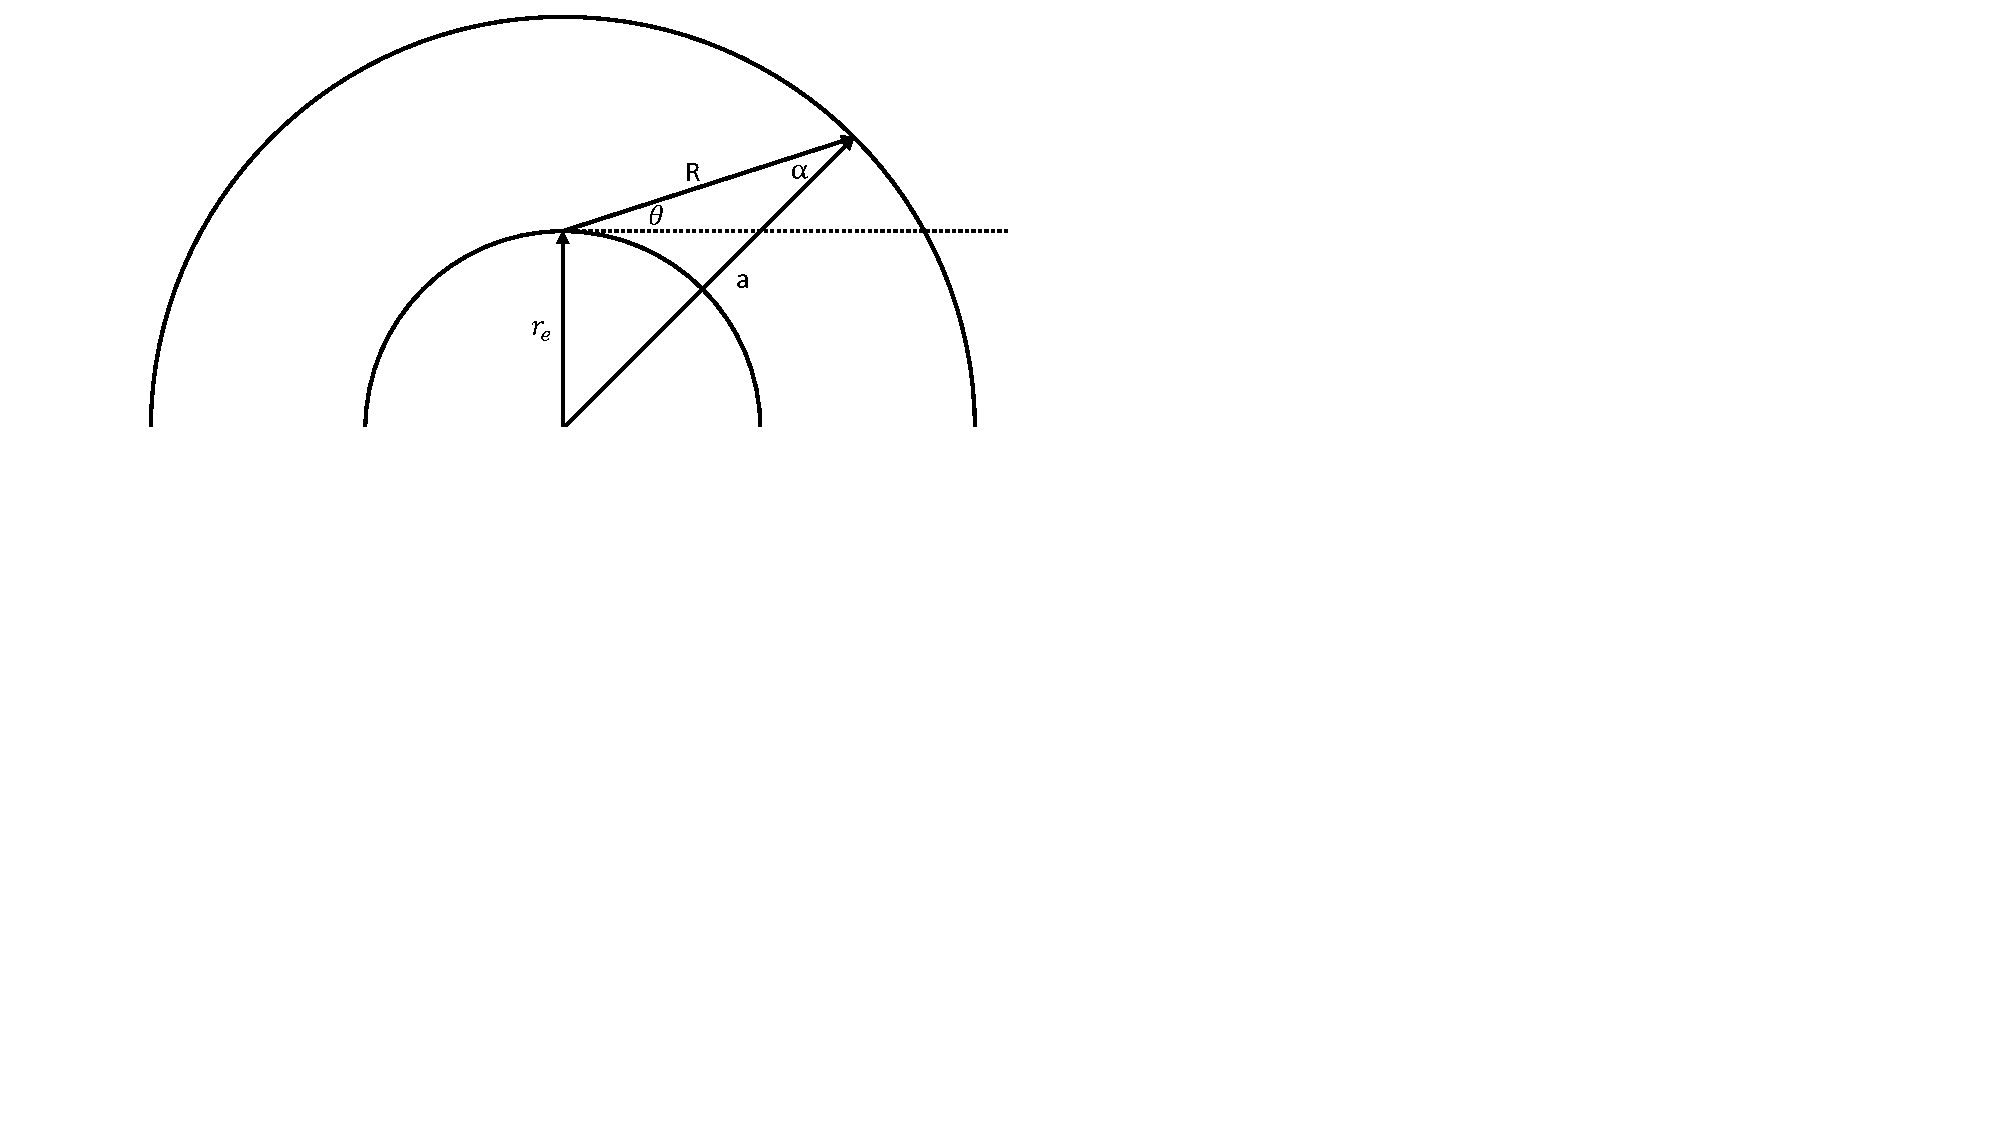
\includegraphics[trim={0 11cm 16cm 0},clip,width = 0.7\linewidth]{ChapterExperiments/Figures/orbit_distance}
\end{figure}

Some configurations will not reflect what can be achieved in our current reality but may be able to in the future. The European GNSS constellation \textit{Galileo} will have 30 satellites operating in tandem with GPS. There are also the constellations GLONASS and Beibo the Russian and Chinese constellations that there may be international cooperation in the future to have all the GNSS constellations operating together in a high density system.